\part{Perception and Attention}
\frame{\partpage}

\begin{frame}{Learning Outcomes}
	In this section you will learn how to...
	
	\begin{itemize}
		\item \textbf{Discuss} different explanations of `perception' and their characteristics
		\item \textbf{Discuss} the importance of perception to HCI and explain how we can exploit
		our understanding of perception in designing game interfaces
		\item \textbf{Discuss} the role of attention in our cognitive processes and explain how human
		attention can be exploited in HCI design
	\end{itemize}
\end{frame}

\begin{frame}{Further Reading}
	\begin{itemize}
		\item Eysenck, M.W. and Keane, M.T. (2000) \textit{Cognitive Psychology: A Student's Handbook}. 4th Edition. Erlbaum Associatates.
		\item Newman, W.M. and Lamming, M.G. (1995) \textit{Interactive System Design}. Addison-Wesley.
		\item Norman, D. (1988) \textit{The Psychology of Everyday Things}. MIT Press.
	\end{itemize}
\end{frame}

\begin{frame}{Further Reading}
	\begin{itemize}
		\item Preece, J., Rogers, Y., Sharp, H., Benyon, D., Holland, S., and Carey, T. (1994) \textit{Human-Computer Interaction}. Addison-Wesley.
		\item Gibson, J.J. (1979) \textit{The Ecological Approach to Visual Perception}. Houghton Mifflin.
		\item Gregory, R.L. (1978) \textit{Eye and Brain: The Psychology of Seeing}. 5th Edition. Weidenfeld and Nicolson.
	\end{itemize}
\end{frame}

\begin{frame}{Perception and Representation}
	\begin{itemize}
		\item Perception covered the sequence of events from the presentation of physical stimulus to the concious (or, indeed, unconcious)
		experience of it.
		\item Two approaches to explain visual perception include:
		\begin{itemize}
			\item Gregory's (1978) \textbf{construcitivist} approach;
			\item and the \textbf{direct perception} approach advanced by Gibson (1979).
		\end{itemize}
	\end{itemize}
\end{frame}

\begin{frame}{Perception and Representation}
	\begin{itemize}
		\item The constructivist approach claims `[person person seeing] constructs a model of the world by transforming, enhancing, distoring, and discarding
		information' (from Preece \textit{et al}, 1994).
		\item In essence, humans construct a world of objects from information in the environment and our own knowledge.
		\item In other words, the images we `see' are not copies of the world, but are `mentally constructed' from our own knowledge and skills in 
		comination with sensory information.
	\end{itemize}
\end{frame}

\begin{frame}{Perception and Representation}
	\begin{itemize}
		\item In contrast, the direct perception approach claims `perception is picking up information from the environment and does not require any
		further processing' (from Perry, 2006, p. 12).
		\item In essence, perception is a direct copy of the environment with information being added or removed for the purpose of meaning making.
		\item In other words, the images we `see' are indeed copies of the world, without any further need for processing, but we may process our perception
		in order to interpret things and make meaning.
	\end{itemize}
\end{frame}

\begin{frame}{Perception and Representation}
	\begin{itemize}
		\item Central to the ecology of the, latter, direct perception approach is the notion of an \textbf{affordance} (Norman, 1988)
		\item What we `see' as the permissable actions or behaviours of a systems, objects, or events is permitted---or \textit{afforded} by that thing---is obvious;
		there is no need for further information processing.
	\end{itemize}
\end{frame}

\begin{frame}{Perception and Representation}
	``...the term affordance refers to the perceived and actual properties of the thing, primarily those fundamental properties that determine just how the thing 
	could possibly be used. [...] Affordances provide strong clues to the operations of things. Plates are for pushing. Knobs are for turning. Slots are for inserting 
	things into. Balls are for throwing or bouncing. When affordances are taken advantage of, the user knows what to do just by looking: no picture, label, or instruction 
	needed.''
	
	\vspace{2ex}
	
	(Norman, 1988, p.9)
\end{frame}

\begin{frame}{Perception and Representation}
	\begin{centering}
		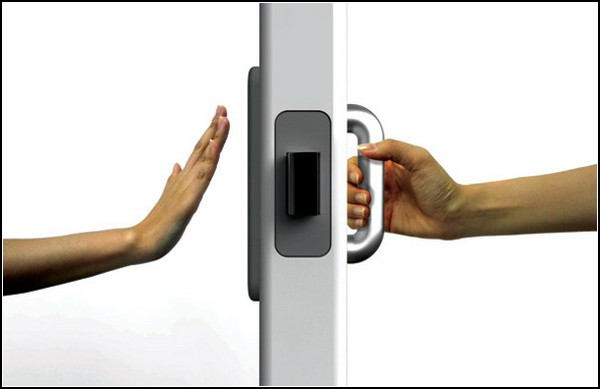
\includegraphics[height=26ex]{door_affordance.jpg}
	\end{centering}
\end{frame}

\begin{frame}{Perception and Representation}
	\begin{centering}
		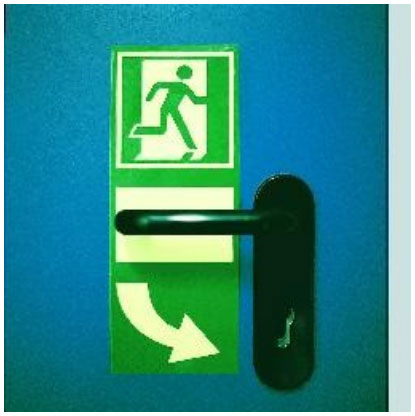
\includegraphics[height=26ex]{guidance_required.jpg}
	\end{centering}
\end{frame}

\begin{frame}{Perception and Representation}
	\begin{itemize}
		\item Affordances are usually viewed an important aspect of the design of game interfaces. It is important to appreciate that affordances are detected---not interpreted.
		\item \textbf{Disambiguation:} A backpack icon for an inventory is a metaphor, not an affordance. This is because it is not obvious how to use it, it has to be interpreted in 
		light of the users' existing knowledge.
	\end{itemize}
\end{frame}

\begin{frame}{Perception and Representation}
	\begin{itemize}
		\item \textbf{Disambiguation:} The escape key to access a menu is a convention, not an affordance. This is because the functionality is premised upon user expectation 
		and therefore requires prior knowledge.
		\item \textbf{Disambiguation:} Solid Snake's wavy bandana illustrating freedom is a semiotic, not an affordance. This is because its a non-verbal sign that communicates 				something and has nothing to do with functionality.
	\end{itemize}
\end{frame}

\begin{frame}[fragile]{Socrative \texttt{JBYPC3BBY}}
	\begin{itemize}
		\item In pairs.
		\item Quietly discuss what affordances exist in game interfaces.
		\item \textbf{List} them.
	\end{itemize}
\end{frame}

\begin{frame}[fragile]{Socrative \texttt{JBYPC3BBY}}
	\begin{columns}[onlytextwidth]
		\begin{column}{0.45\textwidth}
			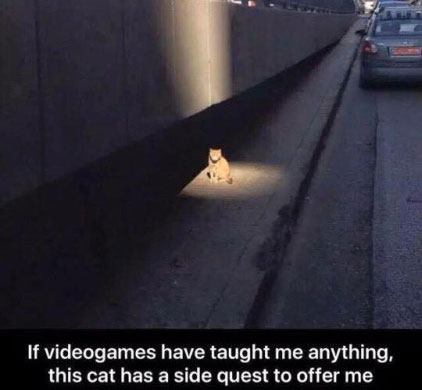
\includegraphics[height=24ex]{quest_cat.jpg}
		\end{column}
		\begin{column}{0.45\textwidth}
			\begin{itemize}
				\item In pairs.
				\item Quietly discuss whether this is an affordance, metaphore, semiotic, or convention.
				\item \textbf{Select} your answer.
			\end{itemize}
		\end{column}
	\end{columns}
\end{frame}

\begin{frame}{Perception and Representation}
	\begin{itemize}
		\item In games, affordances are represented through the interface---often through the pixels. 
		\item As such, they are often illusions. They are not `real' affordances because they have no physical form.
		\item HCI professionals often refer to such affordances as `perceived affordances' due to their virtual nature. They exist only as an artefact of perception.
	\end{itemize}
\end{frame}

\begin{frame}{Perception and Representation}
	\begin{centering}
		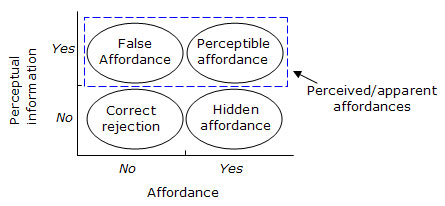
\includegraphics[height=20ex]{false_affordance.jpg}
	\end{centering}
	
	\vspace{2ex}
	
	Caution should be exercised when using perceived affordances due to the risk of creating a false affordance in an interface (Adapted from Norman, 1988).
\end{frame}

\begin{frame}{Perception and Representation}
	We can exploit these artefacts in the design of game interfaces (from Perry, 2006):

	\begin{itemize}
		\item \textbf{Size:} For two similar objects, differing only in size, close together, the larger object will appear much closer than the smaller object. \pause
		\item \textbf{Interposition:} If an object is placed `over' another, such that it is obscured, the unobscured object will appear to sit on top of the other.
	\end{itemize}
\end{frame}

\begin{frame}{Perception and Representation}
	We can exploit these artefacts in the design of game interfaces (from Perry, 2006):

	\begin{itemize}
		\item \textbf{Contrast:} Objects that are further away, gradually dissapring into the distance, appear to lose their contrast, clarity, and brightness; this
		can be simulated in the interface to illustrate relative distances between objects. \pause
		\item \textbf{Texture:} Level of detail of objects appears to grow larger as they come closer. As such, objects with more detail appear closer than those
		with less clearly defined features.
	\end{itemize}
\end{frame}

\begin{frame}{Perception and Representation}
	We can exploit these artefacts in the design of game interfaces (from Perry, 2006):

	\begin{itemize}
		\item \textbf{Shadow:} Placing a shadow behind an object makes it appear to sit above the screen; with changes to shadow size making the `space' behind
		it appear deeper or shallower.
	\end{itemize}
\end{frame}

\begin{frame}{Perception and Representation}
	\begin{itemize}
		\item It is not possible to show all information as directly perceivable physical objects. 
		\item Designers have to consider moving beyond represent\textbf{ed} objects to represent\textbf{ing} abstract forms.
		\item That is, to create symbols: something standing in for something else.
		\item There are two ways this is done in games---direct mappings and arbitrary mappings (from Perry, 2006).
	\end{itemize}
\end{frame}

\begin{frame}{Perception and Representation}
	\begin{itemize}
		\item \textbf{Direct Mapping:} A direct correspondence exists between the objects represented and the form of respresentation. Examples include
		the use of metaphors (e.g. a backpack icon for an inventory) and (some) semiotics (e.g. red to highlight a hostile entity).
	\end{itemize}
\end{frame}

\begin{frame}{Perception and Representation}
	\begin{itemize}
		\item \textbf{Arbitrary Mapping:} No direct link between the object represented and the form of presentation. Examples include the use of abstract
		codes (e.g. 50 for a creeper when using the /summon command), abstract shapes (e.g. $+$ for health), and team colors in multiplayer games. However,
		these abritrary codes need to be learned before they can be used effectively.
	\end{itemize}
\end{frame}

\begin{frame}[fragile]{Socrative \texttt{JBYPC3BBY}}
	\begin{itemize}
		\item In pairs.
		\item Quietly discuss what other \textbf{direct mappings} exist in game interfaces.
		\item \textbf{List} them.
	\end{itemize}
\end{frame}

\begin{frame}[fragile]{Socrative \texttt{JBYPC3BBY}}
	\begin{itemize}
		\item In pairs.
		\item Quietly discuss what other \textbf{arbitrary mappings} exist in game interfaces.
		\item \textbf{List} them.
	\end{itemize}
\end{frame}

\begin{frame}{Colour Perception and Colour Blindness}
	\begin{columns}[onlytextwidth]
		\begin{column}{0.45\textwidth}
			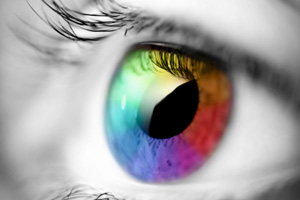
\includegraphics[height=16ex]{normal_vision.jpg}
		\end{column}
		\begin{column}{0.45\textwidth}
			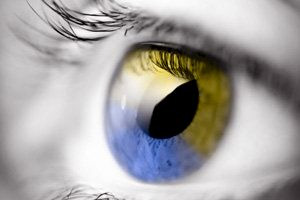
\includegraphics[height=16ex]{anomalous_vision.jpg}
		\end{column}
	\end{columns}
	
	\vspace{2ex}
	
	\begin{itemize}
		\item When designing user interfaces, it is important that we do not arbitrarily exclude users with impairment. 
		\item A common form of visual impairment that affects players is deuteranomaly (8\% of men and 0.5\% of women).
	\end{itemize}
\end{frame}

\begin{frame}{Colour Perception and Colour Blindness}
	\begin{itemize}
		\item Colour coding of interface design elements must take this into account
		\item Examples of common issues can be found at \url{gameaccessibilityguidelines.com}.
	\end{itemize}
\end{frame}

\begin{frame}[fragile]{Socrative \texttt{JBYPC3BBY}}
	\begin{itemize}
		\item In pairs.
		\item Review the guidelines at: \url{gameaccessibilityguidelines.com}.
		\item \textbf{Identify ONE} example of a flaw in a game interface and how to overcome it.
	\end{itemize}
\end{frame}

\begin{frame}{Attention and Memory Constraints}
	\begin{itemize}
		\item At a biological level, humans have capacity constraints that limit the information that they can perceive and process.
		\item To manage this, we tend to converge on two forms of attention:
		\begin{itemize}
			\item \textbf{foused attention}: attending to one event only.
			\item \textbf{divided attention}: multi-tasking
		\end{itemize}	
	\end{itemize}
\end{frame}

\begin{frame}[fragile]{Socrative \texttt{JBYPC3BBY}}
	\begin{itemize}
		\item \textbf{Give} ONE example of a game interface that requires \textbf{focused attention}.
		\item \textbf{Give} ONE example of a game interface that requires \textbf{divided attention}.
	\end{itemize}
\end{frame}

\begin{frame}{Attention and Memory Constraints}
	Several techniques can be used to focus attention in a game interface (adapted from Preece \textit{et al}, 1994):

	\begin{itemize}
		\item \textbf{colour}: colour schemes differentiate areas on the screen, such as the grey side-bar in C\&C games
		\item \textbf{structure}: information is positioned to faciliate ease of access, such as resources positioned on the HUD
		\item \textbf{alerting}: noise and flashing to direct attention, such as the shields down alert in the Halo series
	\end{itemize}
\end{frame}

\begin{frame}{Attention and Memory Constraints}
	Several techniques can be used to focus attention in a game interface (adapted from Preece \textit{et al}, 1994):

	\begin{itemize}
		\item \textbf{highlighting}: information is highlighted at  relevant location, such as the grenade off-screen arrow in Fallout
		\item \textbf{windowing}: information pops up in a window, such as a confirmation dialogue when trading in Guild Wars
	\end{itemize}
\end{frame}
